\documentclass{standalone}
\usepackage{graphicx}	
\usepackage{amssymb, amsmath, amsthm}
\usepackage{color}

\usepackage{tikz}
\usetikzlibrary{intersections, backgrounds}

\definecolor{light}{RGB}{220, 188, 188}
\definecolor{mid}{RGB}{185, 124, 124}
\definecolor{dark}{RGB}{143, 39, 39}
\definecolor{highlight}{RGB}{180, 31, 180}
\definecolor{gray10}{gray}{0.1}
\definecolor{gray20}{gray}{0.2}
\definecolor{gray30}{gray}{0.3}
\definecolor{gray40}{gray}{0.4}
\definecolor{gray60}{gray}{0.6}
\definecolor{gray70}{gray}{0.7}
\definecolor{gray80}{gray}{0.8}
\definecolor{gray90}{gray}{0.9}
\definecolor{gray95}{gray}{0.95}

\begin{document}

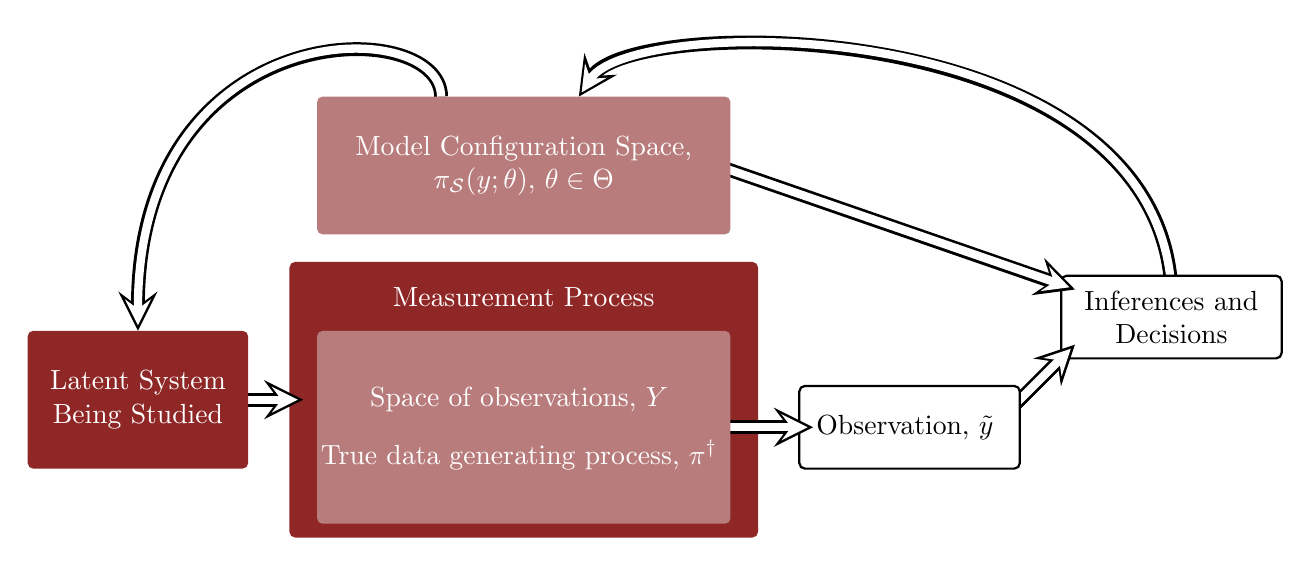
\begin{tikzpicture}[scale=0.35, thick]
  \fill [white] (0, 0) rectangle (45.6, 18.5);
  \clip (0, 0) rectangle (45.6, 18.5);
  
  \draw[->, >=stealth, line width=5] 
    (41.5, 9) .. controls (41, 19) and (22, 19) .. (20, 16);
    
  \draw[->, >=stealth, line width=3, white] 
    (41.5, 9) .. controls (40.9, 19.1) and (22, 19.05) .. (20.1, 16.15);
  
  \draw[->, >=stealth, line width=5] 
    (15, 16) .. controls (15, 19) and (4, 19) .. (4, 7.5);
    
  \draw[->, >=stealth, line width=3, white] 
    (15, 16) .. controls (15, 19) and (4, 19.1) .. (4, 7.7);

  \fill [rounded corners=2pt, color=white] (37.5, 6.5) rectangle (45.5, 9.5);
  \draw [rounded corners=2pt] (37.5, 6.5) rectangle (45.5, 9.5) 
  node[midway, align=center] { Inferences and\\Decisions }; 
  
  \draw[->, >=stealth, line width=5] (35, 4) -- (38, 7);
  \draw[->, >=stealth, line width=3, white] (35, 4) -- (37.85, 6.85);
  
  \draw [rounded corners=2pt, fill=white] (28, 2.5) rectangle (36, 5.5) 
  node[midway, align=center] { Observation, $\tilde{y}$ }; 
  
  \draw[->, >=stealth, line width=5] (25, 13.5) -- (38, 9);
  \draw[->, >=stealth, line width=3, white] (25, 13.5) -- (37.8, 9.08);
  
  \fill [rounded corners=2pt, fill=mid, text=white] (10.5, 11) rectangle (25.5, 16) 
  node[midway, align=center] 
  { Model Configuration Space,\\$\pi_{\mathcal{S}}(y ; \theta), \,\theta \in \Theta$ };
  
  \fill [rounded corners=2pt, fill=dark, text=white] (9.5,0) rectangle (26.5, 10) 
  node [midway, yshift=37, align=center] {Measurement Process};
  
  \draw[->, >=stealth, line width=5] (25.5, 4) -- (28.5, 4);
  \draw[->, >=stealth, line width=3, white] (25.5, 4) -- (28.3, 4);
  
  \fill [rounded corners=2pt, fill=mid, text=white] (10.5, 0.5) rectangle (25.5, 7.5) 
  node[midway, yshift=10, align=center] { Space of observations, $Y$ }
  node[midway, yshift=-10, align=center] { True data generating process, $\pi^{\dagger}$ };

  \draw[->, >=stealth, line width=5] (8, 5) -- (10, 5);
  \draw[->, >=stealth, line width=3, white] (8, 5) -- (9.8, 5);

  \fill [rounded corners=2pt, fill=dark, text=white] (0,2.5) rectangle (8, 7.5) 
  node [midway, align=center] {Latent System\\Being Studied};
  
\end{tikzpicture}

\end{document}  